% 1977 年山东A卷第 1（6）题：正四棱台的三视图——上排为正视图、左视图（两个等腰梯形，带点划线对称轴），下排为俯视图（外大内小两个正方形、四角相连）（按源卷第 2 页布局）
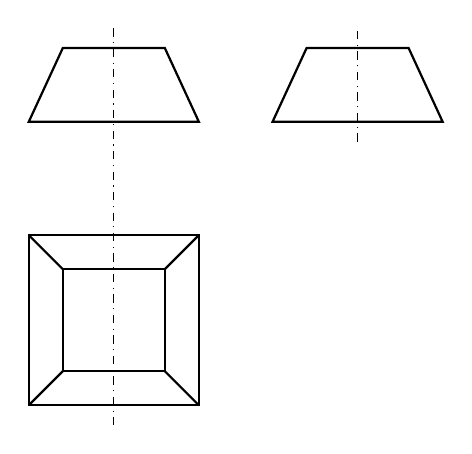
\begin{tikzpicture}[scale=0.72]
  % 正视图（左上）
  \draw[thick] (-1.5,0) -- (1.5,0) -- (0.9,1.3) -- (-0.9,1.3) -- cycle;
  \draw[dashdotted] (0,1.65) -- (0,-5.35);
  % 左视图（右上）
  \begin{scope}[shift={(4.3,0)}]
    \draw[thick] (-1.5,0) -- (1.5,0) -- (0.9,1.3) -- (-0.9,1.3) -- cycle;
    \draw[dashdotted] (0,-0.35) -- (0,1.65);
  \end{scope}
  % 俯视图（左下）
  \draw[thick] (-1.5,-5.0) rectangle (1.5,-2.0);
  \draw[thick] (-0.9,-4.4) rectangle (0.9,-2.6);
  \draw[thick] (-1.5,-2.0) -- (-0.9,-2.6);
  \draw[thick] (1.5,-2.0) -- (0.9,-2.6);
  \draw[thick] (-1.5,-5.0) -- (-0.9,-4.4);
  \draw[thick] (1.5,-5.0) -- (0.9,-4.4);
\end{tikzpicture}
